% Options for packages loaded elsewhere
\PassOptionsToPackage{unicode}{hyperref}
\PassOptionsToPackage{hyphens}{url}
%
\documentclass[
]{article}
\usepackage{amsmath,amssymb}
\usepackage{iftex}
\ifPDFTeX
  \usepackage[T1]{fontenc}
  \usepackage[utf8]{inputenc}
  \usepackage{textcomp} % provide euro and other symbols
\else % if luatex or xetex
  \usepackage{unicode-math} % this also loads fontspec
  \defaultfontfeatures{Scale=MatchLowercase}
  \defaultfontfeatures[\rmfamily]{Ligatures=TeX,Scale=1}
\fi
\usepackage{lmodern}
\ifPDFTeX\else
  % xetex/luatex font selection
\fi
% Use upquote if available, for straight quotes in verbatim environments
\IfFileExists{upquote.sty}{\usepackage{upquote}}{}
\IfFileExists{microtype.sty}{% use microtype if available
  \usepackage[]{microtype}
  \UseMicrotypeSet[protrusion]{basicmath} % disable protrusion for tt fonts
}{}
\makeatletter
\@ifundefined{KOMAClassName}{% if non-KOMA class
  \IfFileExists{parskip.sty}{%
    \usepackage{parskip}
  }{% else
    \setlength{\parindent}{0pt}
    \setlength{\parskip}{6pt plus 2pt minus 1pt}}
}{% if KOMA class
  \KOMAoptions{parskip=half}}
\makeatother
\usepackage{xcolor}
\usepackage[margin=1in]{geometry}
\usepackage{graphicx}
\makeatletter
\newsavebox\pandoc@box
\newcommand*\pandocbounded[1]{% scales image to fit in text height/width
  \sbox\pandoc@box{#1}%
  \Gscale@div\@tempa{\textheight}{\dimexpr\ht\pandoc@box+\dp\pandoc@box\relax}%
  \Gscale@div\@tempb{\linewidth}{\wd\pandoc@box}%
  \ifdim\@tempb\p@<\@tempa\p@\let\@tempa\@tempb\fi% select the smaller of both
  \ifdim\@tempa\p@<\p@\scalebox{\@tempa}{\usebox\pandoc@box}%
  \else\usebox{\pandoc@box}%
  \fi%
}
% Set default figure placement to htbp
\def\fps@figure{htbp}
\makeatother
\setlength{\emergencystretch}{3em} % prevent overfull lines
\providecommand{\tightlist}{%
  \setlength{\itemsep}{0pt}\setlength{\parskip}{0pt}}
\setcounter{secnumdepth}{-\maxdimen} % remove section numbering
\usepackage{booktabs}
\usepackage{longtable}
\usepackage{array}
\usepackage{multirow}
\usepackage{wrapfig}
\usepackage{float}
\usepackage{colortbl}
\usepackage{pdflscape}
\usepackage{tabu}
\usepackage{threeparttable}
\usepackage{threeparttablex}
\usepackage[normalem]{ulem}
\usepackage{makecell}
\usepackage{xcolor}
\usepackage{bookmark}
\IfFileExists{xurl.sty}{\usepackage{xurl}}{} % add URL line breaks if available
\urlstyle{same}
\hypersetup{
  pdftitle={Reglas de Asociación},
  hidelinks,
  pdfcreator={LaTeX via pandoc}}

\title{Reglas de Asociación}
\author{}
\date{\vspace{-2.5em}}

\begin{document}
\maketitle

Con el objetivo de facilitar el análisis de reglas de asociación, se
realizó una transformación de las variables de la base de datos. Las
variables numéricas \texttt{precio} y \texttt{superficie} se agruparon
en cuartiles, generando variables categóricas como ``precio\_bajo'' o
``superficie\_alta''. Asimismo, se transformaron variables booleanas en
etiquetas comprensibles (por ejemplo, \texttt{tieneAscensor\ =\ 1} se
convierte en \texttt{"con\_ascensor"}), eliminando redundancias y
garantizando la consistencia semántica de los datos.

Una vez procesados los datos, se aplicó el algoritmo \textbf{Apriori}
con un umbral mínimo de soporte del 1\% y confianza del 50\% obteniendo
un total de 12745 reglas. Posteriormente se han eliminado reglas
redundantes, aquellas que no aportan información adicional respecto a
reglas más generales con igual o mejor confianza. Esto permite conservar
las reglas más significativas. Las reglas maximales no se han
priorizado, ya que suelen perder especificidad, dificultando su
aplicación práctica. Tras eliminar las redundantes nos quedamos con un
total de 2408 reglas. Por último, filtramos las reglas con los
siguientes umbrales quedándonos con las 21 reglas más relevantes:
Soporte \textgreater{} 0.015, Confianza \textgreater{} 0.7 y Lift
\textgreater{} 3.5

Estas condiciones permiten identificar patrones \textbf{robustos y
estadísticamente relevantes} que relacionan ciertas configuraciones de
un inmueble con su probabilidad de pertenecer a un rango de precio
específico. A continuación se muestran las \textbf{cinco reglas más
destacadas}, ordenadas por su \emph{lift}. Es importante destacar que
las 21 reglas comparten el consecuente de \textbf{Precio Alto}.

\begin{table}[!h]
\centering
\caption{\label{tab:Reglas Precio Alto}Reglas de asociación más relevantes (ordenadas por lift)}
\centering
\resizebox{\ifdim\width>\linewidth\linewidth\else\width\fi}{!}{
\begin{tabular}[t]{l|l|r|r|r|r|r}
\hline
  & rules & support & confidence & coverage & lift & count\\
\hline
1001 & \{rooms\_4+\_habitaciones,tieneAscensor\_con\_ascensor,bathrooms\_3+\_banios\} => \{priceAmount\_precio\_alto\} & 0.017 & 0.970 & 0.018 & 3.879 & 32\\
\hline
8593 & \{surface\_surface\_alto,tieneAscensor\_con\_ascensor,tieneAireAcondicionado\_con\_aire,bathrooms\_3+\_banios,tieneCalefaccion\_con\_calefaccion\} => \{priceAmount\_precio\_alto\} & 0.017 & 0.970 & 0.018 & 3.879 & 32\\
\hline
4075 & \{surface\_surface\_alto,tieneAscensor\_con\_ascensor,tieneAireAcondicionado\_con\_aire,bathrooms\_3+\_banios\} => \{priceAmount\_precio\_alto\} & 0.022 & 0.952 & 0.023 & 3.810 & 40\\
\hline
4063 & \{surface\_surface\_alto,tieneAscensor\_con\_ascensor,bathrooms\_3+\_banios,tieneCalefaccion\_con\_calefaccion\} => \{priceAmount\_precio\_alto\} & 0.018 & 0.943 & 0.019 & 3.771 & 33\\
\hline
4087 & \{tieneAscensor\_con\_ascensor,tieneAireAcondicionado\_con\_aire,bathrooms\_3+\_banios,tieneCalefaccion\_con\_calefaccion\} => \{priceAmount\_precio\_alto\} & 0.018 & 0.943 & 0.019 & 3.771 & 33\\
\hline
\end{tabular}}
\end{table}

Una vez identificadas dichas reglas y analizando que están asociadas a
precios altos, exploramos ahora aquellas cuya consecuencia es
priceAmount = precio\_bajo. Este tipo de reglas resulta especialmente
útil para detectar inmuebles infravalorados o con condiciones objetivas
que los hacen significativamente más asequibles. Para ello, filtramos
las reglas con: Soporte \textgreater{} 0.0107, Confianza \textgreater{}
0.8 y Lift \textgreater{} 2.7

\begin{table}[!h]
\centering
\caption{\label{tab:Reglas Precio Bajo}Reglas de asociación más relevantes asociadas a Precios Bajos (ordenadas por lift)}
\centering
\resizebox{\ifdim\width>\linewidth\linewidth\else\width\fi}{!}{
\begin{tabular}[t]{l|l|r|r|r|r|r}
\hline
  & rules & support & confidence & coverage & lift & count\\
\hline
4271 & \{tieneAscensor\_sin\_ascensor,rooms\_1\_habitacion,surface\_surface\_bajo,tieneAireAcondicionado\_sin\_aire\} => \{priceAmount\_precio\_bajo\} & 0.011 & 0.840 & 0.013 & 3.360 & 21\\
\hline
8705 & \{tieneTrastero\_sin\_trastero,tieneCalefaccion\_sin\_calefaccion,rooms\_1\_habitacion,surface\_surface\_bajo,tieneAireAcondicionado\_sin\_aire\} => \{priceAmount\_precio\_bajo\} & 0.012 & 0.821 & 0.015 & 3.286 & 23\\
\hline
4284 & \{tieneCalefaccion\_sin\_calefaccion,rooms\_1\_habitacion,surface\_surface\_bajo,tieneAireAcondicionado\_sin\_aire\} => \{priceAmount\_precio\_bajo\} & 0.013 & 0.806 & 0.017 & 3.226 & 25\\
\hline
\end{tabular}}
\end{table}

A continuación, se han empleado gráficos para explorar visualmente las
reglas de asociación: un \textbf{diagrama de dispersión (scatter plot)}
para analizar la relación entre soporte y confianza, y un
\textbf{gráfico de coordenadas paralelas} para examinar la estructura
interna de las reglas en términos de los atributos que las componen. No
se utilizaron representaciones como el grouped matrix ni la matriz de
calor, ya que estas técnicas son más adecuadas cuando las reglas
implican combinaciones simples entre pocos ítems. Al estar las reglas
formadas por múltiples atributos simultáneos, genera una gran
dimensionalidad y dificulta la interpretación gráfica en formatos
matriciales. Por ello, se optó por visualizaciones más eficaces para
este tipo de complejidad estructural.

\begin{figure}[H]

{\centering 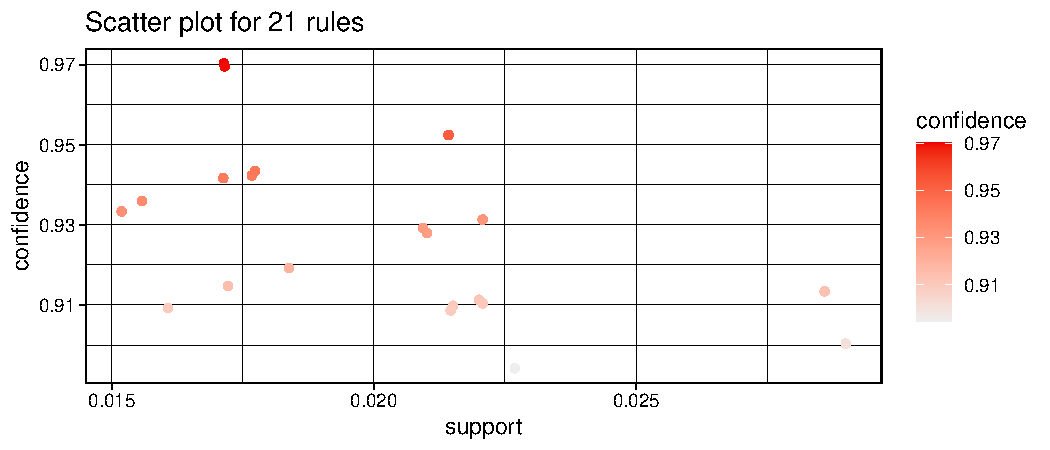
\includegraphics{reglas_asociacion_resumen_v2_files/figure-latex/Grafico Dispersion-1} 

}

\caption{Distribución de Reglas}\label{fig:Grafico Dispersion}
\end{figure}

El gráfico de dispersión muestra la relación entre el soporte y la
confianza de las 21 reglas de asociación seleccionadas, con una escala
de color que representa el nivel de confianza. Comprobamos que todas las
reglas tienen un soporte comprendido entre 0.015 y 0.025, lo cual indica
que aunque no son extremadamente frecuentes, sí aparecen con suficiente
consistencia en la base de datos. En términos de confianza, todas
superan el umbral mínimo de 0.7, alcanzando valores próximos al 0.97.
Esto indica que cuando se cumplen las condiciones del antecedente, la
probabilidad de que el precio sea alto es muy elevada. Las reglas con
mayor confianza tienden a tener un soporte ligeramente menor, lo que
sugiere que, si bien son altamente fiables, aplican a un subconjunto más
específico del mercado inmobiliario.

\begin{figure}[H]

{\centering 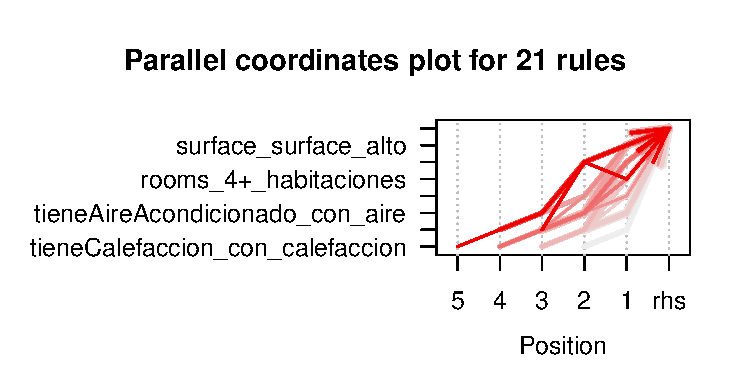
\includegraphics{reglas_asociacion_resumen_v2_files/figure-latex/Coordenadas Paralelas-1} 

}

\caption{Gráfico de Coordenadas Paralelas}\label{fig:Coordenadas Paralelas}
\end{figure}

El gráfico de coordenadas paralelas representa visualmente la estructura
interna de las reglas más representativas. Cada línea corresponde a una
regla individual, y su recorrido conecta los distintos atributos que
forman el antecedente, finalizando en el consecuente
(priceAmount\_precio\_alto).

Se aprecia una clara convergencia de reglas hacia ciertos atributos
comunes, como:

\begin{itemize}
\item
  Superficie elevada del inmueble (surface\_surface\_alto)
\item
  Existencia de ascensor (tieneAscensor\_con\_ascensor)
\item
  Más de 3 baños (bathrooms\_3+\_banios)
\item
  Existencia de calefacción (tieneCalefaccion\_con\_calefaccion)
\end{itemize}

Estas características aparecen reiteradamente como predictores del
precio alto, lo que refuerza su relevancia dentro del conjunto de datos
analizado.

Este análisis ha revelado patrones sólidos entre las características
estructurales de los inmuebles y su rango de precio. En particular,
propiedades con gran superficie, múltiples baños y habitaciones,
ascensor, calefacción y aire acondicionado muestran una alta
probabilidad de pertenecer al segmento de precio alto.

\end{document}
